\documentclass[]{article}
\usepackage{lmodern}
\usepackage{amssymb,amsmath}
\usepackage{ifxetex,ifluatex}
\usepackage{fixltx2e} % provides \textsubscript
\ifnum 0\ifxetex 1\fi\ifluatex 1\fi=0 % if pdftex
  \usepackage[T1]{fontenc}
  \usepackage[utf8]{inputenc}
\else % if luatex or xelatex
  \ifxetex
    \usepackage{mathspec}
  \else
    \usepackage{fontspec}
  \fi
  \defaultfontfeatures{Ligatures=TeX,Scale=MatchLowercase}
\fi
% use upquote if available, for straight quotes in verbatim environments
\IfFileExists{upquote.sty}{\usepackage{upquote}}{}
% use microtype if available
\IfFileExists{microtype.sty}{%
\usepackage{microtype}
\UseMicrotypeSet[protrusion]{basicmath} % disable protrusion for tt fonts
}{}
\usepackage[margin=1in]{geometry}
\usepackage{hyperref}
\hypersetup{unicode=true,
            pdftitle={Quantitative Analyst with R},
            pdfauthor={Manuela Chadreque},
            pdfborder={0 0 0},
            breaklinks=true}
\urlstyle{same}  % don't use monospace font for urls
\usepackage{color}
\usepackage{fancyvrb}
\newcommand{\VerbBar}{|}
\newcommand{\VERB}{\Verb[commandchars=\\\{\}]}
\DefineVerbatimEnvironment{Highlighting}{Verbatim}{commandchars=\\\{\}}
% Add ',fontsize=\small' for more characters per line
\usepackage{framed}
\definecolor{shadecolor}{RGB}{248,248,248}
\newenvironment{Shaded}{\begin{snugshade}}{\end{snugshade}}
\newcommand{\KeywordTok}[1]{\textcolor[rgb]{0.13,0.29,0.53}{\textbf{#1}}}
\newcommand{\DataTypeTok}[1]{\textcolor[rgb]{0.13,0.29,0.53}{#1}}
\newcommand{\DecValTok}[1]{\textcolor[rgb]{0.00,0.00,0.81}{#1}}
\newcommand{\BaseNTok}[1]{\textcolor[rgb]{0.00,0.00,0.81}{#1}}
\newcommand{\FloatTok}[1]{\textcolor[rgb]{0.00,0.00,0.81}{#1}}
\newcommand{\ConstantTok}[1]{\textcolor[rgb]{0.00,0.00,0.00}{#1}}
\newcommand{\CharTok}[1]{\textcolor[rgb]{0.31,0.60,0.02}{#1}}
\newcommand{\SpecialCharTok}[1]{\textcolor[rgb]{0.00,0.00,0.00}{#1}}
\newcommand{\StringTok}[1]{\textcolor[rgb]{0.31,0.60,0.02}{#1}}
\newcommand{\VerbatimStringTok}[1]{\textcolor[rgb]{0.31,0.60,0.02}{#1}}
\newcommand{\SpecialStringTok}[1]{\textcolor[rgb]{0.31,0.60,0.02}{#1}}
\newcommand{\ImportTok}[1]{#1}
\newcommand{\CommentTok}[1]{\textcolor[rgb]{0.56,0.35,0.01}{\textit{#1}}}
\newcommand{\DocumentationTok}[1]{\textcolor[rgb]{0.56,0.35,0.01}{\textbf{\textit{#1}}}}
\newcommand{\AnnotationTok}[1]{\textcolor[rgb]{0.56,0.35,0.01}{\textbf{\textit{#1}}}}
\newcommand{\CommentVarTok}[1]{\textcolor[rgb]{0.56,0.35,0.01}{\textbf{\textit{#1}}}}
\newcommand{\OtherTok}[1]{\textcolor[rgb]{0.56,0.35,0.01}{#1}}
\newcommand{\FunctionTok}[1]{\textcolor[rgb]{0.00,0.00,0.00}{#1}}
\newcommand{\VariableTok}[1]{\textcolor[rgb]{0.00,0.00,0.00}{#1}}
\newcommand{\ControlFlowTok}[1]{\textcolor[rgb]{0.13,0.29,0.53}{\textbf{#1}}}
\newcommand{\OperatorTok}[1]{\textcolor[rgb]{0.81,0.36,0.00}{\textbf{#1}}}
\newcommand{\BuiltInTok}[1]{#1}
\newcommand{\ExtensionTok}[1]{#1}
\newcommand{\PreprocessorTok}[1]{\textcolor[rgb]{0.56,0.35,0.01}{\textit{#1}}}
\newcommand{\AttributeTok}[1]{\textcolor[rgb]{0.77,0.63,0.00}{#1}}
\newcommand{\RegionMarkerTok}[1]{#1}
\newcommand{\InformationTok}[1]{\textcolor[rgb]{0.56,0.35,0.01}{\textbf{\textit{#1}}}}
\newcommand{\WarningTok}[1]{\textcolor[rgb]{0.56,0.35,0.01}{\textbf{\textit{#1}}}}
\newcommand{\AlertTok}[1]{\textcolor[rgb]{0.94,0.16,0.16}{#1}}
\newcommand{\ErrorTok}[1]{\textcolor[rgb]{0.64,0.00,0.00}{\textbf{#1}}}
\newcommand{\NormalTok}[1]{#1}
\usepackage{graphicx,grffile}
\makeatletter
\def\maxwidth{\ifdim\Gin@nat@width>\linewidth\linewidth\else\Gin@nat@width\fi}
\def\maxheight{\ifdim\Gin@nat@height>\textheight\textheight\else\Gin@nat@height\fi}
\makeatother
% Scale images if necessary, so that they will not overflow the page
% margins by default, and it is still possible to overwrite the defaults
% using explicit options in \includegraphics[width, height, ...]{}
\setkeys{Gin}{width=\maxwidth,height=\maxheight,keepaspectratio}
\IfFileExists{parskip.sty}{%
\usepackage{parskip}
}{% else
\setlength{\parindent}{0pt}
\setlength{\parskip}{6pt plus 2pt minus 1pt}
}
\setlength{\emergencystretch}{3em}  % prevent overfull lines
\providecommand{\tightlist}{%
  \setlength{\itemsep}{0pt}\setlength{\parskip}{0pt}}
\setcounter{secnumdepth}{0}
% Redefines (sub)paragraphs to behave more like sections
\ifx\paragraph\undefined\else
\let\oldparagraph\paragraph
\renewcommand{\paragraph}[1]{\oldparagraph{#1}\mbox{}}
\fi
\ifx\subparagraph\undefined\else
\let\oldsubparagraph\subparagraph
\renewcommand{\subparagraph}[1]{\oldsubparagraph{#1}\mbox{}}
\fi

%%% Use protect on footnotes to avoid problems with footnotes in titles
\let\rmarkdownfootnote\footnote%
\def\footnote{\protect\rmarkdownfootnote}

%%% Change title format to be more compact
\usepackage{titling}

% Create subtitle command for use in maketitle
\newcommand{\subtitle}[1]{
  \posttitle{
    \begin{center}\large#1\end{center}
    }
}

\setlength{\droptitle}{-2em}
  \title{Quantitative Analyst with R}
  \pretitle{\vspace{\droptitle}\centering\huge}
  \posttitle{\par}
  \author{Manuela Chadreque}
  \preauthor{\centering\large\emph}
  \postauthor{\par}
  \predate{\centering\large\emph}
  \postdate{\par}
  \date{11 de MarÃf§o de 2019}


\begin{document}
\maketitle

\section{instal and load packedges}\label{instal-and-load-packedges}

\subsection{Introduction to R for
Finance!}\label{introduction-to-r-for-finance}

\subsubsection{The Basics}\label{the-basics}

\paragraph{Arithmetic in R}\label{arithmetic-in-r}

Addition: + Subtraction: - Multiplication: * Division: / Exponentiation:
\^{} or ** Modulo: \%\%

\begin{Shaded}
\begin{Highlighting}[]
\CommentTok{# Addition }
\DecValTok{2} \OperatorTok{+}\StringTok{ }\DecValTok{2}
\end{Highlighting}
\end{Shaded}

\begin{verbatim}
## [1] 4
\end{verbatim}

\begin{Shaded}
\begin{Highlighting}[]
\CommentTok{# Subtraction}
\DecValTok{4} \OperatorTok{-}\StringTok{ }\DecValTok{1}
\end{Highlighting}
\end{Shaded}

\begin{verbatim}
## [1] 3
\end{verbatim}

\begin{Shaded}
\begin{Highlighting}[]
\CommentTok{# Multiplication}
\DecValTok{3} \OperatorTok{*}\StringTok{ }\DecValTok{4}
\end{Highlighting}
\end{Shaded}

\begin{verbatim}
## [1] 12
\end{verbatim}

\begin{Shaded}
\begin{Highlighting}[]
\CommentTok{# Division}

\DecValTok{4}\OperatorTok{/}\DecValTok{2}
\end{Highlighting}
\end{Shaded}

\begin{verbatim}
## [1] 2
\end{verbatim}

\begin{Shaded}
\begin{Highlighting}[]
\CommentTok{# Exponentiation}

\DecValTok{2}\OperatorTok{^}\DecValTok{4}
\end{Highlighting}
\end{Shaded}

\begin{verbatim}
## [1] 16
\end{verbatim}

\begin{Shaded}
\begin{Highlighting}[]
\CommentTok{# Modulo}
\DecValTok{7}\OperatorTok\DecValTok{3}
\end{Highlighting}
\end{Shaded}

\begin{verbatim}
## [1] 1
\end{verbatim}

\subsubsection{Assignment and variables}\label{assignment-and-variables}

A variable allows you to store a value or an object in R. You can then
later use this variable's name to easily access the value or the object
that is stored within this variable. You use \textless{}- to assign a
variable:

my\_money \textless{}- 100

\begin{Shaded}
\begin{Highlighting}[]
\CommentTok{# Assign 200 to savings}
\NormalTok{savings <-}\StringTok{ }\DecValTok{200}

\CommentTok{# Print the value of savings to the console}
\NormalTok{savings}
\end{Highlighting}
\end{Shaded}

\begin{verbatim}
## [1] 200
\end{verbatim}

\paragraph{Aritmetrics with variables}\label{aritmetrics-with-variables}

\begin{Shaded}
\begin{Highlighting}[]
\CommentTok{# Assign 100 to my_money}
\NormalTok{my_money <-}\StringTok{ }\DecValTok{100}

\CommentTok{# Assign 200 to dans_money}
\NormalTok{dans_money<-}\DecValTok{200}

\CommentTok{# Add my_money and dans_money}
\NormalTok{my_money}\OperatorTok{+}\NormalTok{dans_money}
\end{Highlighting}
\end{Shaded}

\begin{verbatim}
## [1] 300
\end{verbatim}

\begin{Shaded}
\begin{Highlighting}[]
\CommentTok{# Add my_money and dans_money again, save the result to our_money}
\NormalTok{our_money<-my_money}\OperatorTok{+}\NormalTok{dans_money}
\KeywordTok{print}\NormalTok{(our_money)}
\end{Highlighting}
\end{Shaded}

\begin{verbatim}
## [1] 300
\end{verbatim}

\section{Financial returns}\label{financial-returns}

Assume you have \$100. During January, you make a 5\% return on that
money. How much do you have at the end of January? Well, you have 100\%
of your starting money, plus another 5\%: 100\% + 5\% = 105\%. In
decimals, this is 1 + .05 = 1.05. This 1.05 is the return multiplier for
January, and you multiply your original \$100 by it to get the amount
you have at the end of January.

105 = 100 * 1.05

Or in terms of variables:

post\_jan\_cash \textless{}- starting\_cash * jan\_ret

A quick way to get the multiplier is:

multiplier = 1 + (return / 100) If, in February, you earn another 2\% on
your cash, how would you calculate the total amount at the end of
February? You already know that the amount at the end of January is
\$100 * 1.05 = \$105. To get from the end of January to the end of
February, just use another multiplier!

\$105 * 1.02 = \$107.1

Which is equivalent to:

\$100 * 1.05 * 1.02 = \$107.1

\begin{Shaded}
\begin{Highlighting}[]
\CommentTok{# Variables for starting_cash and 5% return during January}
\NormalTok{starting_cash <-}\StringTok{ }\DecValTok{200}
\NormalTok{jan_ret <-}\StringTok{ }\DecValTok{5}
\NormalTok{jan_mult <-}\StringTok{ }\DecValTok{1} \OperatorTok{+}\StringTok{ }\NormalTok{(jan_ret }\OperatorTok{/}\StringTok{ }\DecValTok{100}\NormalTok{)}

\CommentTok{# How much money do you have at the end of January?}
\NormalTok{post_jan_cash <-}\StringTok{ }\NormalTok{starting_cash}\OperatorTok{*}\NormalTok{jan_mult}

\CommentTok{# Print post_jan_cash}
\NormalTok{post_jan_cash}
\end{Highlighting}
\end{Shaded}

\begin{verbatim}
## [1] 210
\end{verbatim}

\begin{Shaded}
\begin{Highlighting}[]
\CommentTok{# January 10% return multiplier}
\NormalTok{jan_ret_}\DecValTok{10}\NormalTok{ <-}\StringTok{ }\DecValTok{10}
\NormalTok{jan_mult_}\DecValTok{10}\NormalTok{ <-}\StringTok{ }\DecValTok{1}\OperatorTok{+}\NormalTok{(jan_ret_}\DecValTok{10}\OperatorTok{/}\DecValTok{100}\NormalTok{)}

\CommentTok{# How much money do you have at the end of January now?}
\NormalTok{post_jan_cash_}\DecValTok{10}\NormalTok{ <-}\StringTok{ }\NormalTok{starting_cash}\OperatorTok{*}\NormalTok{jan_mult_}\DecValTok{10}


\CommentTok{# Print post_jan_cash_10}
\NormalTok{post_jan_cash_}\DecValTok{10}
\end{Highlighting}
\end{Shaded}

\begin{verbatim}
## [1] 220
\end{verbatim}

\begin{Shaded}
\begin{Highlighting}[]
\CommentTok{# Starting cash and returns }
\NormalTok{starting_cash <-}\StringTok{ }\DecValTok{200}
\NormalTok{jan_ret <-}\StringTok{ }\DecValTok{4}
\NormalTok{feb_ret <-}\StringTok{ }\DecValTok{5}

\CommentTok{# Multipliers}
\NormalTok{jan_mult <-}\StringTok{ }\DecValTok{1}\OperatorTok{+}\NormalTok{(jan_ret}\OperatorTok{/}\DecValTok{100}\NormalTok{)}
\NormalTok{feb_mult <-}\StringTok{ }\DecValTok{1}\OperatorTok{+}\NormalTok{feb_ret}\OperatorTok{/}\DecValTok{100}

\CommentTok{# Total cash at the end of the two months}
\NormalTok{total_cash <-}\StringTok{ }\NormalTok{starting_cash}\OperatorTok{*}\NormalTok{jan_mult}\OperatorTok{*}\NormalTok{feb_mult}

\CommentTok{# Print total_cash}
\NormalTok{total_cash}
\end{Highlighting}
\end{Shaded}

\begin{verbatim}
## [1] 218.4
\end{verbatim}

\subsubsection{Data type exploration}\label{data-type-exploration}

To get started, here are some of R's most basic data types:

Numerics are decimal numbers like 4.5. A special type of numeric is an
integer, which is a numeric without a decimal piece. Integers must be
specified like 4L. Logicals are the boolean values TRUE and FALSE.
Capital letters are important here; true and false are not valid.
Characters are text values like ``hello world''.

\paragraph{What's that data type?}\label{whats-that-data-type}

Up until now, you have been determining what data type a variable is
just by looks. There is actually a better way to check this.

class(my\_var)

\begin{Shaded}
\begin{Highlighting}[]
\CommentTok{# }
\CommentTok{# # company's stock price is a numeric}
\CommentTok{# company_stock <- 150.45}
\CommentTok{# }
\CommentTok{# # Bond credit ratings are characters}
\CommentTok{# credit_rating <-"AAA"}
\CommentTok{# }
\CommentTok{# # You like the stock market. TRUE or FALSE?}
\CommentTok{# my_answer <- TRUE}
\CommentTok{# }
\CommentTok{# # Print my_answer}
\CommentTok{# my_answer}
\end{Highlighting}
\end{Shaded}

\subsubsection{Vector}\label{vector}

\paragraph{c()ombine}\label{combine}

Now is where things get fun! It is time to create your first vector.
Since this is a finance oriented course, it is only appropriate that
your first vector be a numeric vector of stock prices. Remember, you
create a vector using the combine function, c(), and each element you
add is separated by a comma. We can also add names to each return in
your vector. You do this using names()

\begin{Shaded}
\begin{Highlighting}[]
\CommentTok{# Another numeric vector}
\NormalTok{ibm_stock <-}\StringTok{ }\KeywordTok{c}\NormalTok{(}\FloatTok{159.82}\NormalTok{, }\FloatTok{160.02}\NormalTok{, }\FloatTok{159.84}\NormalTok{)}

\CommentTok{# Another character vector}
\NormalTok{finance <-}\KeywordTok{c}\NormalTok{(}\StringTok{"stocks"}\NormalTok{, }\StringTok{"bonds"}\NormalTok{, }\StringTok{"investments"}\NormalTok{)}

\CommentTok{# A logical vector}
\NormalTok{logic <-}\StringTok{ }\KeywordTok{c}\NormalTok{(}\OtherTok{TRUE}\NormalTok{,}\OtherTok{FALSE}\NormalTok{,}\OtherTok{TRUE}\NormalTok{)}


\CommentTok{# Vectors of 12 months of returns, and month names}
\NormalTok{ret <-}\StringTok{ }\KeywordTok{c}\NormalTok{(}\DecValTok{5}\NormalTok{, }\DecValTok{2}\NormalTok{, }\DecValTok{3}\NormalTok{, }\DecValTok{7}\NormalTok{, }\DecValTok{8}\NormalTok{, }\DecValTok{3}\NormalTok{, }\DecValTok{5}\NormalTok{, }\DecValTok{9}\NormalTok{, }\DecValTok{1}\NormalTok{, }\DecValTok{4}\NormalTok{, }\DecValTok{6}\NormalTok{, }\DecValTok{3}\NormalTok{)}
\NormalTok{months <-}\StringTok{ }\KeywordTok{c}\NormalTok{(}\StringTok{"Jan"}\NormalTok{, }\StringTok{"Feb"}\NormalTok{, }\StringTok{"Mar"}\NormalTok{, }\StringTok{"Apr"}\NormalTok{, }\StringTok{"May"}\NormalTok{, }\StringTok{"Jun"}\NormalTok{, }\StringTok{"Jul"}\NormalTok{, }\StringTok{"Aug"}\NormalTok{, }\StringTok{"Sep"}\NormalTok{, }\StringTok{"Oct"}\NormalTok{, }\StringTok{"Nov"}\NormalTok{, }\StringTok{"Dec"}\NormalTok{)}

\CommentTok{# Add names to ret}
\KeywordTok{names}\NormalTok{(ret) <-}\StringTok{ }\NormalTok{months}

\CommentTok{# Print out ret to see the new names!}
\NormalTok{ret}
\end{Highlighting}
\end{Shaded}

\begin{verbatim}
## Jan Feb Mar Apr May Jun Jul Aug Sep Oct Nov Dec 
##   5   2   3   7   8   3   5   9   1   4   6   3
\end{verbatim}

\subsubsection{Visualize your vector}\label{visualize-your-vector}

The plot() function is one of the many ways to create a graph from your
data in R. Passing in a vector will add its values to the y-axis of the
graph, and on the x-axis will be an index created from the order that
your vector is in.

Inside of plot(), you can change the type of your graph using type =.
The default is ``p'' for points, but you can also change it to ``l'' for
line.

\begin{Shaded}
\begin{Highlighting}[]
\NormalTok{apple_stock <-}\StringTok{ }\KeywordTok{c}\NormalTok{(}\FloatTok{109.49}\NormalTok{, }\FloatTok{109.90}\NormalTok{, }\FloatTok{109.11}\NormalTok{, }\FloatTok{109.95}\NormalTok{, }\FloatTok{111.03}\NormalTok{, }\FloatTok{112.12}\NormalTok{)}
\NormalTok{credit_rating <-}\StringTok{ }\KeywordTok{c}\NormalTok{(}\StringTok{"AAA"}\NormalTok{, }\StringTok{"AA"}\NormalTok{, }\StringTok{"BBB"}\NormalTok{, }\StringTok{"BB"}\NormalTok{, }\StringTok{"B"}\NormalTok{)}
\NormalTok{micr<-}\KeywordTok{c}\NormalTok{(}\FloatTok{59.20}\NormalTok{,}\FloatTok{59.25}\NormalTok{,}\FloatTok{60.22}\NormalTok{,}\FloatTok{59.95}\NormalTok{,}\FloatTok{61.37}\NormalTok{,}\FloatTok{61.01}\NormalTok{,}\FloatTok{61.97}\NormalTok{,}\FloatTok{62.17}\NormalTok{,}\FloatTok{62.98}\NormalTok{,}\FloatTok{62.68}\NormalTok{,}\FloatTok{62.58}\NormalTok{,}\FloatTok{62.30}
\NormalTok{,}\FloatTok{63.62}\NormalTok{,}\FloatTok{63.54}\NormalTok{,}\FloatTok{63.54}\NormalTok{,}\FloatTok{63.55}\NormalTok{,}\FloatTok{63.24}\NormalTok{,}\FloatTok{63.28}\NormalTok{,}\FloatTok{62.99}\NormalTok{,}\FloatTok{62.90}\NormalTok{,}\FloatTok{62.14}\NormalTok{)}

\CommentTok{# Look at the data}
\NormalTok{apple_stock}
\end{Highlighting}
\end{Shaded}

\begin{verbatim}
## [1] 109.49 109.90 109.11 109.95 111.03 112.12
\end{verbatim}

\begin{Shaded}
\begin{Highlighting}[]
\CommentTok{# Plot the data points}
\KeywordTok{plot}\NormalTok{(apple_stock)}
\end{Highlighting}
\end{Shaded}

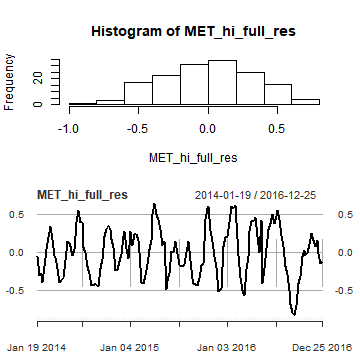
\includegraphics{Introduction_to_R_for_Finance_files/figure-latex/unnamed-chunk-7-1.pdf}

\begin{Shaded}
\begin{Highlighting}[]
\CommentTok{# Plot the data as a line graph}
\KeywordTok{plot}\NormalTok{(apple_stock, }\DataTypeTok{type =} \StringTok{"l"}\NormalTok{)}
\end{Highlighting}
\end{Shaded}

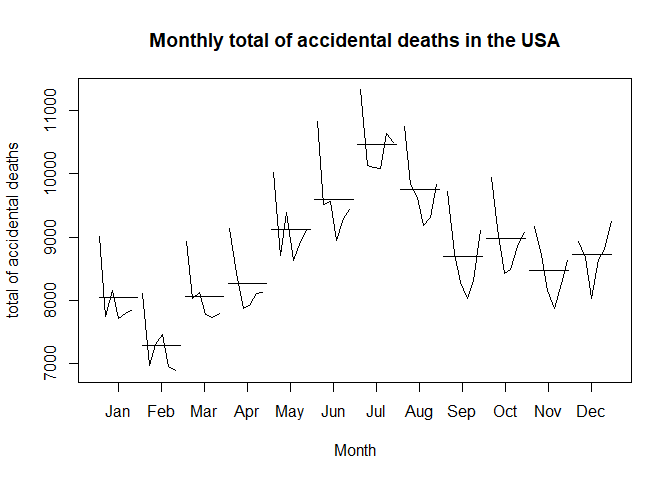
\includegraphics{Introduction_to_R_for_Finance_files/figure-latex/unnamed-chunk-7-2.pdf}
\#\#\#\#Weighted average As a finance professional, there are a number
of important calculations that you will have to know. One of these is
the weighted average. The weighted average allows you to calculate your
portfolio return over a time period. Consider the following example:

Assume you have 40\% of your cash in Apple stock, and 60\% of your cash
in IBM stock. If, in January, Apple earned 5\% and IBM earned 7\%, what
was your total portfolio return?

To calculate this, take the return of each stock in your portfolio, and
multiply it by the weight of that stock. Then sum up all of the results.
For this example, you would do:

6.2 = 5 * .4 + 7 * .6

Or, in variable terms:

portf\_ret \textless{}- apple\_ret * apple\_weight + ibm\_ret *
ibm\_weight

\begin{Shaded}
\begin{Highlighting}[]
\CommentTok{# Weights and returns}
\NormalTok{micr_ret<-}\StringTok{ }\DecValTok{7}
\NormalTok{sony_ret <-}\StringTok{ }\DecValTok{9}
\NormalTok{micr_weight <-}\StringTok{ }\NormalTok{.}\DecValTok{2}
\NormalTok{sony_weight <-}\StringTok{ }\NormalTok{.}\DecValTok{8}

\CommentTok{# Portfolio return}
\NormalTok{portf_ret <-micr_ret }\OperatorTok{*}\StringTok{ }\NormalTok{micr_weight }\OperatorTok{+}\StringTok{ }\NormalTok{sony_ret }\OperatorTok{*}\StringTok{ }\NormalTok{sony_weight}


\CommentTok{# Weights, returns, and company names}
\NormalTok{ret <-}\StringTok{ }\KeywordTok{c}\NormalTok{(}\DecValTok{7}\NormalTok{, }\DecValTok{9}\NormalTok{)}
\NormalTok{weight <-}\StringTok{ }\KeywordTok{c}\NormalTok{(.}\DecValTok{2}\NormalTok{, .}\DecValTok{8}\NormalTok{)}
\NormalTok{companies <-}\StringTok{ }\KeywordTok{c}\NormalTok{(}\StringTok{"Microsoft"}\NormalTok{, }\StringTok{"Sony"}\NormalTok{)}

\CommentTok{# Assign company names to your vectors}
\KeywordTok{names}\NormalTok{(ret) <-}\StringTok{ }\NormalTok{companies}
\KeywordTok{names}\NormalTok{(weight) <-}\StringTok{ }\NormalTok{companies}

\CommentTok{# Multiply the returns and weights together }
\NormalTok{ret_X_weight <-}\StringTok{ }\NormalTok{ret}\OperatorTok{*}\NormalTok{weight}

\CommentTok{# Print ret_X_weight}
\NormalTok{ret_X_weight}
\end{Highlighting}
\end{Shaded}

\begin{verbatim}
## Microsoft      Sony 
##       1.4       7.2
\end{verbatim}

\begin{Shaded}
\begin{Highlighting}[]
\CommentTok{# Sum to get the total portfolio return}
\NormalTok{portf_ret <-}\KeywordTok{sum}\NormalTok{(ret_X_weight)}

\CommentTok{# Print portf_ret}
\KeywordTok{sum}\NormalTok{(portf_ret)}
\end{Highlighting}
\end{Shaded}

\begin{verbatim}
## [1] 8.6
\end{verbatim}

\begin{Shaded}
\begin{Highlighting}[]
\CommentTok{# Print ret}
\NormalTok{ret }
\end{Highlighting}
\end{Shaded}

\begin{verbatim}
## Microsoft      Sony 
##         7         9
\end{verbatim}

\begin{Shaded}
\begin{Highlighting}[]
\CommentTok{# Assign 1/3 to weight}
\NormalTok{weight <-}\StringTok{ }\DecValTok{1}\OperatorTok{/}\DecValTok{3}

\CommentTok{# Create ret_X_weight}
\NormalTok{ret_X_weight <-}\StringTok{ }\NormalTok{ret}\OperatorTok{*}\NormalTok{weight}

\CommentTok{# Calculate your portfolio return}
\NormalTok{portf_ret <-}\StringTok{ }\KeywordTok{sum}\NormalTok{(ret_X_weight)}

\CommentTok{# Vector of length 3 * Vector of length 2?}
\NormalTok{ret }\OperatorTok{*}\StringTok{ }\KeywordTok{c}\NormalTok{(.}\DecValTok{2}\NormalTok{, .}\DecValTok{6}\NormalTok{)}
\end{Highlighting}
\end{Shaded}

\begin{verbatim}
## Microsoft      Sony 
##       1.4       5.4
\end{verbatim}

\paragraph{Vector subsetting}\label{vector-subsetting}

Sometimes, you will only want to use specific pieces of your vectors,
and you'll need some way to access just those parts. For example, what
if you only wanted the first month of returns from the vector of 12
months of returns? To solve this, you can subset the vector using {[}
{]}.

Here is the 12 month return vector:

ret \textless{}- c(5, 2, 3, 7, 8, 3, 5, 9, 1, 4, 6, 3)

Select the first month: ret{[}1{]}.

Select the first month by name: ret{[}``Jan''{]}.

Select the first three months: ret{[}1:3{]} or ret{[}c(1, 2, 3){]}.

\begin{Shaded}
\begin{Highlighting}[]
\NormalTok{ret <-}\StringTok{ }\KeywordTok{c}\NormalTok{(}\DecValTok{5}\NormalTok{, }\DecValTok{2}\NormalTok{, }\DecValTok{3}\NormalTok{, }\DecValTok{7}\NormalTok{, }\DecValTok{8}\NormalTok{, }\DecValTok{3}\NormalTok{, }\DecValTok{5}\NormalTok{, }\DecValTok{9}\NormalTok{, }\DecValTok{1}\NormalTok{, }\DecValTok{4}\NormalTok{, }\DecValTok{6}\NormalTok{, }\DecValTok{3}\NormalTok{)}

\CommentTok{# First 6 months of returns}
\NormalTok{ret[}\DecValTok{1}\OperatorTok{:}\DecValTok{6}\NormalTok{]}
\end{Highlighting}
\end{Shaded}

\begin{verbatim}
## [1] 5 2 3 7 8 3
\end{verbatim}

\begin{Shaded}
\begin{Highlighting}[]
\CommentTok{# Just March and May}
\NormalTok{ret[}\KeywordTok{c}\NormalTok{(}\StringTok{"Mar"}\NormalTok{,}\StringTok{"May"}\NormalTok{)]}
\end{Highlighting}
\end{Shaded}

\begin{verbatim}
## [1] NA NA
\end{verbatim}

\begin{Shaded}
\begin{Highlighting}[]
\CommentTok{# Omit the first month of returns}
\NormalTok{ret[}\OperatorTok{-}\DecValTok{1}\NormalTok{]}
\end{Highlighting}
\end{Shaded}

\begin{verbatim}
##  [1] 2 3 7 8 3 5 9 1 4 6 3
\end{verbatim}

\subsubsection{Matrix}\label{matrix}

Matrices are similar to vectors, except they are in 2 dimensions! Let's
create a 2x2 matrix ``by hand'' using matrix().

\begin{Shaded}
\begin{Highlighting}[]
\CommentTok{# A vector of 9 numbers}
\NormalTok{my_vector <-}\StringTok{ }\KeywordTok{c}\NormalTok{(}\DecValTok{1}\NormalTok{, }\DecValTok{2}\NormalTok{, }\DecValTok{3}\NormalTok{, }\DecValTok{4}\NormalTok{, }\DecValTok{5}\NormalTok{, }\DecValTok{6}\NormalTok{, }\DecValTok{7}\NormalTok{, }\DecValTok{8}\NormalTok{, }\DecValTok{9}\NormalTok{)}

\CommentTok{# 3x3 matrix}
\NormalTok{my_matrix <-}\StringTok{ }\KeywordTok{matrix}\NormalTok{(}\DataTypeTok{data =}\NormalTok{ my_vector, }\DataTypeTok{nrow =} \DecValTok{3}\NormalTok{, }\DataTypeTok{ncol =}\DecValTok{3}\NormalTok{)}

\CommentTok{# Print my_matrix}
\NormalTok{my_matrix}
\end{Highlighting}
\end{Shaded}

\begin{verbatim}
##      [,1] [,2] [,3]
## [1,]    1    4    7
## [2,]    2    5    8
## [3,]    3    6    9
\end{verbatim}

\begin{Shaded}
\begin{Highlighting}[]
\CommentTok{# Filling across using byrow = TRUE}
\NormalTok{apple_micr_matrix<-}\KeywordTok{matrix}\NormalTok{(}\DataTypeTok{data =} \KeywordTok{c}\NormalTok{(}\DecValTok{2}\NormalTok{, }\DecValTok{3}\NormalTok{, }\DecValTok{4}\NormalTok{, }\DecValTok{5}\NormalTok{), }\DataTypeTok{nrow =} \DecValTok{2}\NormalTok{, }\DataTypeTok{ncol =} \DecValTok{2}\NormalTok{, }\DataTypeTok{byrow =} \OtherTok{TRUE}\NormalTok{)}

\CommentTok{# View the data}
\NormalTok{apple_micr_matrix}
\end{Highlighting}
\end{Shaded}

\begin{verbatim}
##      [,1] [,2]
## [1,]    2    3
## [2,]    4    5
\end{verbatim}

\begin{Shaded}
\begin{Highlighting}[]
\CommentTok{# Scatter plot of Microsoft vs Apple}
\KeywordTok{plot}\NormalTok{(apple_micr_matrix)}
\end{Highlighting}
\end{Shaded}

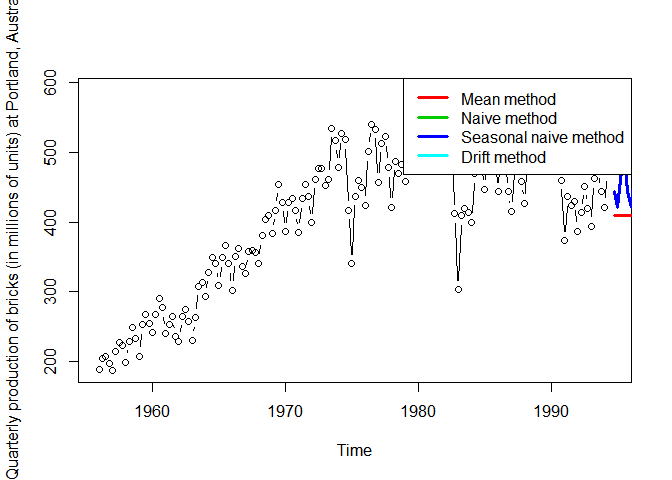
\includegraphics{Introduction_to_R_for_Finance_files/figure-latex/unnamed-chunk-10-1.pdf}
\#\#\#cor()relation The cor() function will calculate the correlation
between two vectors, or will create a correlation matrix when given a
matrix.

\begin{Shaded}
\begin{Highlighting}[]
\NormalTok{apple <-}\StringTok{ }\KeywordTok{c}\NormalTok{(}\FloatTok{109.49}\NormalTok{, }\FloatTok{109.90}\NormalTok{, }\FloatTok{109.11}\NormalTok{, }\FloatTok{109.95}\NormalTok{, }\FloatTok{111.03}\NormalTok{)}
\NormalTok{ibm <-}\StringTok{ }\KeywordTok{c}\NormalTok{(}\FloatTok{159.82}\NormalTok{, }\FloatTok{160.02}\NormalTok{, }\FloatTok{159.84}\NormalTok{, }\FloatTok{160.35}\NormalTok{, }\FloatTok{164.79}\NormalTok{)}

\CommentTok{# cbind the vectors together}
\NormalTok{cbind_stocks <-}\StringTok{ }\KeywordTok{cbind}\NormalTok{(apple,ibm,micr)}
\end{Highlighting}
\end{Shaded}

\begin{verbatim}
## Warning in cbind(apple, ibm, micr): number of rows of result is not a
## multiple of vector length (arg 1)
\end{verbatim}

\begin{Shaded}
\begin{Highlighting}[]
\CommentTok{# Print cbind_stocks}
\NormalTok{cbind_stocks}
\end{Highlighting}
\end{Shaded}

\begin{verbatim}
##        apple    ibm  micr
##  [1,] 109.49 159.82 59.20
##  [2,] 109.90 160.02 59.25
##  [3,] 109.11 159.84 60.22
##  [4,] 109.95 160.35 59.95
##  [5,] 111.03 164.79 61.37
##  [6,] 109.49 159.82 61.01
##  [7,] 109.90 160.02 61.97
##  [8,] 109.11 159.84 62.17
##  [9,] 109.95 160.35 62.98
## [10,] 111.03 164.79 62.68
## [11,] 109.49 159.82 62.58
## [12,] 109.90 160.02 62.30
## [13,] 109.11 159.84 63.62
## [14,] 109.95 160.35 63.54
## [15,] 111.03 164.79 63.54
## [16,] 109.49 159.82 63.55
## [17,] 109.90 160.02 63.24
## [18,] 109.11 159.84 63.28
## [19,] 109.95 160.35 62.99
## [20,] 111.03 164.79 62.90
## [21,] 109.49 159.82 62.14
\end{verbatim}

\begin{Shaded}
\begin{Highlighting}[]
\CommentTok{# rbind the vectors together}
\NormalTok{rbind_stocks <-}\StringTok{ }\KeywordTok{rbind}\NormalTok{(apple,ibm,micr)}
\end{Highlighting}
\end{Shaded}

\begin{verbatim}
## Warning in rbind(apple, ibm, micr): number of columns of result is not a
## multiple of vector length (arg 1)
\end{verbatim}

\begin{Shaded}
\begin{Highlighting}[]
\CommentTok{# Print rbind_stocks}
\NormalTok{rbind_stocks}
\end{Highlighting}
\end{Shaded}

\begin{verbatim}
##         [,1]   [,2]   [,3]   [,4]   [,5]   [,6]   [,7]   [,8]   [,9]
## apple 109.49 109.90 109.11 109.95 111.03 109.49 109.90 109.11 109.95
## ibm   159.82 160.02 159.84 160.35 164.79 159.82 160.02 159.84 160.35
## micr   59.20  59.25  60.22  59.95  61.37  61.01  61.97  62.17  62.98
##        [,10]  [,11]  [,12]  [,13]  [,14]  [,15]  [,16]  [,17]  [,18]
## apple 111.03 109.49 109.90 109.11 109.95 111.03 109.49 109.90 109.11
## ibm   164.79 159.82 160.02 159.84 160.35 164.79 159.82 160.02 159.84
## micr   62.68  62.58  62.30  63.62  63.54  63.54  63.55  63.24  63.28
##        [,19]  [,20]  [,21]
## apple 109.95 111.03 109.49
## ibm   160.35 164.79 159.82
## micr   62.99  62.90  62.14
\end{verbatim}

\subsubsection{Matrix subsetting}\label{matrix-subsetting}

Matrix subsetting Just like vectors, matrices can be selected from and
subsetted! To do this, you will again use {[} {]}, but this time it will
have two inputs. The basic structure is:

my\_matrix{[}row, col{]}

Then: To select the first row and first column of stocks from the last
example: stocks{[}1,1{]}

To select the entire first row, leave the col empty: stocks{[}1, {]}

To select the first two rows: stocks{[}1:2, {]} or stocks{[}c(1,2), {]}

To select an entire column, leave the row empty: stocks{[}, 1{]}

You can also select an entire column by name: stocks{[}, ``apple''{]}

\begin{Shaded}
\begin{Highlighting}[]
\NormalTok{stocks<-cbind_stocks}
\CommentTok{# Third row}
\NormalTok{stocks[}\DecValTok{3}\NormalTok{,]}
\end{Highlighting}
\end{Shaded}

\begin{verbatim}
##  apple    ibm   micr 
## 109.11 159.84  60.22
\end{verbatim}

\begin{Shaded}
\begin{Highlighting}[]
\CommentTok{# Fourth and fifth row of the ibm column}
\NormalTok{stocks[}\KeywordTok{c}\NormalTok{(}\DecValTok{4}\NormalTok{,}\DecValTok{5}\NormalTok{),}\StringTok{"ibm"}\NormalTok{]}
\end{Highlighting}
\end{Shaded}

\begin{verbatim}
## [1] 160.35 164.79
\end{verbatim}

\begin{Shaded}
\begin{Highlighting}[]
\CommentTok{# apple and micr columns}
\NormalTok{stocks[,}\KeywordTok{c}\NormalTok{(}\StringTok{"apple"}\NormalTok{,}\StringTok{"micr"}\NormalTok{)]}
\end{Highlighting}
\end{Shaded}

\begin{verbatim}
##        apple  micr
##  [1,] 109.49 59.20
##  [2,] 109.90 59.25
##  [3,] 109.11 60.22
##  [4,] 109.95 59.95
##  [5,] 111.03 61.37
##  [6,] 109.49 61.01
##  [7,] 109.90 61.97
##  [8,] 109.11 62.17
##  [9,] 109.95 62.98
## [10,] 111.03 62.68
## [11,] 109.49 62.58
## [12,] 109.90 62.30
## [13,] 109.11 63.62
## [14,] 109.95 63.54
## [15,] 111.03 63.54
## [16,] 109.49 63.55
## [17,] 109.90 63.24
## [18,] 109.11 63.28
## [19,] 109.95 62.99
## [20,] 111.03 62.90
## [21,] 109.49 62.14
\end{verbatim}

\subsubsection{data.frame()}\label{data.frame}

Data frames are great because of their ability to hold a different type
of data in each column. To get started, let's use the data.frame()
function to create a data frame of your business's future cash flows.
Here are the variables that will be in the data frame:

company - The company that is paying you the cash flow (A or B).
cash\_flow - The amount of money a company will receive. year - The
number of years from now that you receive the cash flow.

\begin{Shaded}
\begin{Highlighting}[]
\CommentTok{# Variables}
\NormalTok{company <-}\StringTok{ }\KeywordTok{c}\NormalTok{(}\StringTok{"A"}\NormalTok{, }\StringTok{"A"}\NormalTok{, }\StringTok{"A"}\NormalTok{, }\StringTok{"B"}\NormalTok{, }\StringTok{"B"}\NormalTok{, }\StringTok{"B"}\NormalTok{, }\StringTok{"B"}\NormalTok{)}
\NormalTok{cash_flow <-}\StringTok{ }\KeywordTok{c}\NormalTok{(}\DecValTok{1000}\NormalTok{, }\DecValTok{4000}\NormalTok{, }\DecValTok{550}\NormalTok{, }\DecValTok{1500}\NormalTok{, }\DecValTok{1100}\NormalTok{, }\DecValTok{750}\NormalTok{, }\DecValTok{6000}\NormalTok{)}
\NormalTok{year <-}\StringTok{ }\KeywordTok{c}\NormalTok{(}\DecValTok{1}\NormalTok{, }\DecValTok{3}\NormalTok{, }\DecValTok{4}\NormalTok{, }\DecValTok{1}\NormalTok{, }\DecValTok{2}\NormalTok{, }\DecValTok{4}\NormalTok{, }\DecValTok{5}\NormalTok{)}

\CommentTok{# Data frame}
\NormalTok{cash <-}\StringTok{ }\KeywordTok{data.frame}\NormalTok{(company,cash_flow,year)}

\CommentTok{# Print cash}
\NormalTok{cash}
\end{Highlighting}
\end{Shaded}

\begin{verbatim}
##   company cash_flow year
## 1       A      1000    1
## 2       A      4000    3
## 3       A       550    4
## 4       B      1500    1
## 5       B      1100    2
## 6       B       750    4
## 7       B      6000    5
\end{verbatim}

\subsubsection{Making head()s and tail()s of your data with some
str()ucture}\label{making-heads-and-tails-of-your-data-with-some-structure}

Time to introduce a few simple, but very useful functions.

head() - Returns the first few rows of a data frame. By default, 6. To
change this, use head(cash, n = \textbf{\emph{) tail() - Returns the
last few rows of a data frame. By default, 6. To change this, use
tail(cash, n = }}) str() - Check the structure of an object. This
fantastic function will show you the data type of the object you pass in
(here, data.frame), and will list each column variable along with its
data type. With a small data set such as yours, head() and tail() are
not incredibly useful, but imagine if you had a data frame of hundreds
or thousands of rows!

\begin{Shaded}
\begin{Highlighting}[]
\CommentTok{# Call head() for the first 4 rows}
\KeywordTok{head}\NormalTok{(cash,}\DataTypeTok{n=}\DecValTok{4}\NormalTok{)}
\end{Highlighting}
\end{Shaded}

\begin{verbatim}
##   company cash_flow year
## 1       A      1000    1
## 2       A      4000    3
## 3       A       550    4
## 4       B      1500    1
\end{verbatim}

\begin{Shaded}
\begin{Highlighting}[]
\CommentTok{# Call tail() for the last 3 rows}
\KeywordTok{tail}\NormalTok{(cash,}\DataTypeTok{n=}\DecValTok{3}\NormalTok{)}
\end{Highlighting}
\end{Shaded}

\begin{verbatim}
##   company cash_flow year
## 5       B      1100    2
## 6       B       750    4
## 7       B      6000    5
\end{verbatim}

\begin{Shaded}
\begin{Highlighting}[]
\CommentTok{# Call str()}
\KeywordTok{str}\NormalTok{(cash)}
\end{Highlighting}
\end{Shaded}

\begin{verbatim}
## 'data.frame':    7 obs. of  3 variables:
##  $ company  : Factor w/ 2 levels "A","B": 1 1 1 2 2 2 2
##  $ cash_flow: num  1000 4000 550 1500 1100 750 6000
##  $ year     : num  1 3 4 1 2 4 5
\end{verbatim}

\paragraph{Naming your columns / rows}\label{naming-your-columns-rows}

\begin{Shaded}
\begin{Highlighting}[]
\CommentTok{# Fix your column names}
\KeywordTok{colnames}\NormalTok{(cash)<-}\KeywordTok{c}\NormalTok{(}\StringTok{"company"}\NormalTok{,}\StringTok{"cash_flow"}\NormalTok{,}\StringTok{"year"}\NormalTok{)}

\CommentTok{# Print out the column names of cash}
\KeywordTok{names}\NormalTok{(cash)}
\end{Highlighting}
\end{Shaded}

\begin{verbatim}
## [1] "company"   "cash_flow" "year"
\end{verbatim}

\paragraph{Accessing and subsetting data frames
(1)}\label{accessing-and-subsetting-data-frames-1}

Even more often than with vectors, you are going to want to subset your
data frame or access certain columns. Again, one of the ways to do this
is to use {[} {]}. The notation is just like matrices! Here are some
examples:

Select the first row: cash{[}1, {]}

Select the first column: cash{[} ,1{]}

Select the first column by name: cash{[} ,``company''{]}

Accessing and subsetting data frames (2) As you might imagine, selecting
a specific column from a data frame is a common manipulation. So common,
in fact, that it was given its own shortcut, the \$. The following
return the same answer:

cash\$cash\_flow

{[}1{]} 1000 4000 550 1500 1100 750 6000

cash{[},``cash\_flow''{]}

{[}1{]} 1000 4000 550 1500 1100 750 6000 Accessing and subsetting data
frames (3) Often, just simply selecting a column from a data frame is
not all you want to do. What if you are only interested in the cash
flows from company A? For more flexibility, try subset()!

subset(cash, company == ``A'')

company cash\_flow year 1 A 1000 1 2 A 4000 3 3 A 550 4

\begin{Shaded}
\begin{Highlighting}[]
\CommentTok{# Third row, second column}
\NormalTok{cash[}\DecValTok{3}\NormalTok{,}\DecValTok{2}\NormalTok{]}
\end{Highlighting}
\end{Shaded}

\begin{verbatim}
## [1] 550
\end{verbatim}

\begin{Shaded}
\begin{Highlighting}[]
\CommentTok{# Fifth row of the "year" column}
\NormalTok{cash[}\DecValTok{5}\NormalTok{,}\StringTok{"year"}\NormalTok{]}
\end{Highlighting}
\end{Shaded}

\begin{verbatim}
## [1] 2
\end{verbatim}

\begin{Shaded}
\begin{Highlighting}[]
\CommentTok{# Select the year column}
\NormalTok{cash}\OperatorTok{$}\NormalTok{year}
\end{Highlighting}
\end{Shaded}

\begin{verbatim}
## [1] 1 3 4 1 2 4 5
\end{verbatim}

\begin{Shaded}
\begin{Highlighting}[]
\CommentTok{# Select the cash_flow column and multiply by 2}
\NormalTok{cash}\OperatorTok{$}\NormalTok{cash_flow}\OperatorTok{*}\DecValTok{2}
\end{Highlighting}
\end{Shaded}

\begin{verbatim}
## [1]  2000  8000  1100  3000  2200  1500 12000
\end{verbatim}

\begin{Shaded}
\begin{Highlighting}[]
\CommentTok{# Delete the company column}
\NormalTok{cash}\OperatorTok{$}\NormalTok{company <-}\StringTok{ }\OtherTok{NULL}

\CommentTok{# Print cash again}
\NormalTok{cash}
\end{Highlighting}
\end{Shaded}

\begin{verbatim}
##   cash_flow year
## 1      1000    1
## 2      4000    3
## 3       550    4
## 4      1500    1
## 5      1100    2
## 6       750    4
## 7      6000    5
\end{verbatim}

\begin{Shaded}
\begin{Highlighting}[]
\CommentTok{# Rows about company B}
\KeywordTok{subset}\NormalTok{(cash,company}\OperatorTok{==}\StringTok{"B"}\NormalTok{)}
\end{Highlighting}
\end{Shaded}

\begin{verbatim}
##   cash_flow year
## 4      1500    1
## 5      1100    2
## 6       750    4
## 7      6000    5
\end{verbatim}

\begin{Shaded}
\begin{Highlighting}[]
\CommentTok{# Rows with cash flows due in 1 year}
\KeywordTok{subset}\NormalTok{(cash,year}\OperatorTok{==}\DecValTok{1}\NormalTok{)}
\end{Highlighting}
\end{Shaded}

\begin{verbatim}
##   cash_flow year
## 1      1000    1
## 4      1500    1
\end{verbatim}

\subsubsection{Adding new columns}\label{adding-new-columns}

In a perfect world, you could be 100\% certain that you will receive all
of your cash flows. But, since these are predictions about the future,
there is always a chance that someone won't be able to pay! You decide
to run some analysis about a worst case scenario where you only receive
half of your expected cash flow. To save the worst case scenario for
later analysis, you decide to add it as a new column to the data frame!

cash\(half_cash <- cash\)cash\_flow * .5

cash

company cash\_flow year half\_cash 1 A 1000 1 500 2 A 4000 3 2000 3 A
550 4 275 4 B 1500 1 750 5 B 1100 2 550 6 B 750 4 375 7 B 6000 5 3000

\begin{Shaded}
\begin{Highlighting}[]
\CommentTok{# Quarter cash flow scenario}
\NormalTok{cash}\OperatorTok{$}\NormalTok{quarter_cash <-cash}\OperatorTok{$}\NormalTok{cash_flow}\OperatorTok{*}\FloatTok{0.25}

\CommentTok{# Double year scenario}
\NormalTok{cash}\OperatorTok{$}\NormalTok{double_year<-cash}\OperatorTok{$}\NormalTok{year}\OperatorTok{*}\DecValTok{2}
\end{Highlighting}
\end{Shaded}

\subsubsection{Present value of projected cash
flows}\label{present-value-of-projected-cash-flows}

If you expect a cash flow of \$100 to be received 1 year from now, what
is the present value of that cash flow at a 5\% interest rate? To
calculate this, you discount the cash flow to get it in terms of today's
dollars. The general formula for this is:

present\_value \textless{}- cash\_flow * (1 + interest / 100) \^{} -year

95.238 = 100 * (1.05) \^{} -1

Another way to think about this is to reverse the problem. If you have
\$95.238 today, and it earns 5\% over the next year, how much money do
you have at the end of the year? We know how to do this problem from way
back in chapter 1! Find the multiplier that corresponds to 5\% and
multiply by \$95.238!

100 = 95.238 * (1.05)

\begin{Shaded}
\begin{Highlighting}[]
\CommentTok{# Present value of $4000, in 3 years, at 5%}
\NormalTok{present_value_4k <-}\StringTok{ }\DecValTok{4000}\OperatorTok{*}\NormalTok{(}\DecValTok{1}\OperatorTok{+}\FloatTok{0.05}\NormalTok{)}\OperatorTok{^-}\DecValTok{3}

\CommentTok{# Present value of all cash flows}
\NormalTok{cash}\OperatorTok{$}\NormalTok{present_value <-cash}\OperatorTok{$}\NormalTok{cash_flow}\OperatorTok{*}\NormalTok{(}\DecValTok{1}\OperatorTok{+}\FloatTok{0.05}\NormalTok{)}\OperatorTok{^-}\NormalTok{cash}\OperatorTok{$}\NormalTok{year}

\CommentTok{# Print out cash}
\NormalTok{cash}
\end{Highlighting}
\end{Shaded}

\begin{verbatim}
##   cash_flow year quarter_cash double_year present_value
## 1      1000    1        250.0           2      952.3810
## 2      4000    3       1000.0           6     3455.3504
## 3       550    4        137.5           8      452.4864
## 4      1500    1        375.0           2     1428.5714
## 5      1100    2        275.0           4      997.7324
## 6       750    4        187.5           8      617.0269
## 7      6000    5       1500.0          10     4701.1570
\end{verbatim}

\begin{Shaded}
\begin{Highlighting}[]
\CommentTok{# Total present value of cash}
\NormalTok{total_pv <-}\StringTok{ }\KeywordTok{sum}\NormalTok{(cash}\OperatorTok{$}\NormalTok{present_value)}

\CommentTok{# Company B information}
\NormalTok{cash_B <-}\StringTok{ }\KeywordTok{subset}\NormalTok{(cash,company}\OperatorTok{==}\StringTok{"B"}\NormalTok{)}

\CommentTok{# Total present value of cash_B}
\NormalTok{total_pv_B <-}\StringTok{ }\KeywordTok{sum}\NormalTok{(cash_B}\OperatorTok{$}\NormalTok{present_value)}
\end{Highlighting}
\end{Shaded}

\subsubsection{Factor}\label{factor}

Bond credit ratings are common in the fixed income side of the finance
world as a simple measure of how ``risky'' a certain bond might be.
Here, riskiness can be defined as the probability of default, which
means an inability to pay back your debts. The Standard and Poor's and
Fitch credit rating agency has defined the following ratings, from least
likely to default to most likely:

AAA, AA, A, BBB, BB, B, CCC, CC, C, D This is a perfect example of a
factor! It is a categorical variable that takes on a limited number of
levels.

To create a factor in R, use the factor() function, and pass in a vector
that you want to be converted into a factor.

Suppose you have a portfolio of 7 bonds with these credit ratings:

credit\_rating \textless{}- c(``AAA'', ``AA'', ``A'', ``BBB'', ``AA'',
``BBB'', ``A'')

To create a factor from this:

factor(credit\_rating)

{[}1{]} AAA AA A BBB AA BBB A\\
Levels: A AA AAA BBB

\begin{Shaded}
\begin{Highlighting}[]
\CommentTok{# credit_rating character vector}
\NormalTok{credit_rating <-}\StringTok{ }\KeywordTok{c}\NormalTok{(}\StringTok{"BB"}\NormalTok{, }\StringTok{"AAA"}\NormalTok{, }\StringTok{"AA"}\NormalTok{, }\StringTok{"CCC"}\NormalTok{, }\StringTok{"AA"}\NormalTok{, }\StringTok{"AAA"}\NormalTok{, }\StringTok{"B"}\NormalTok{, }\StringTok{"BB"}\NormalTok{)}

\CommentTok{# Create a factor from credit_rating}
\NormalTok{credit_factor <-}\StringTok{ }\KeywordTok{factor}\NormalTok{(credit_rating)}

\CommentTok{# Print out your new factor}
\NormalTok{credit_factor}
\end{Highlighting}
\end{Shaded}

\begin{verbatim}
## [1] BB  AAA AA  CCC AA  AAA B   BB 
## Levels: AA AAA B BB CCC
\end{verbatim}

\begin{Shaded}
\begin{Highlighting}[]
\CommentTok{# Call str() on credit_rating}
\KeywordTok{str}\NormalTok{(credit_rating)}
\end{Highlighting}
\end{Shaded}

\begin{verbatim}
##  chr [1:8] "BB" "AAA" "AA" "CCC" "AA" "AAA" "B" "BB"
\end{verbatim}

\begin{Shaded}
\begin{Highlighting}[]
\CommentTok{# Call str() on credit_factor}
\KeywordTok{str}\NormalTok{(credit_factor)}
\end{Highlighting}
\end{Shaded}

\begin{verbatim}
##  Factor w/ 5 levels "AA","AAA","B",..: 4 2 1 5 1 2 3 4
\end{verbatim}

\begin{Shaded}
\begin{Highlighting}[]
\CommentTok{# Identify unique levels}
\KeywordTok{levels}\NormalTok{(credit_factor)}
\end{Highlighting}
\end{Shaded}

\begin{verbatim}
## [1] "AA"  "AAA" "B"   "BB"  "CCC"
\end{verbatim}

\begin{Shaded}
\begin{Highlighting}[]
\CommentTok{# Rename the levels of credit_factor}
\KeywordTok{levels}\NormalTok{(credit_factor)<-}\KeywordTok{c}\NormalTok{(}\StringTok{"2A"}\NormalTok{,}\StringTok{"3A"}\NormalTok{,}\StringTok{"1B"}\NormalTok{,}\StringTok{"2B"}\NormalTok{,}\StringTok{"3C"}\NormalTok{)}

\CommentTok{# Print credit_factor}
\NormalTok{credit_factor}
\end{Highlighting}
\end{Shaded}

\begin{verbatim}
## [1] 2B 3A 2A 3C 2A 3A 1B 2B
## Levels: 2A 3A 1B 2B 3C
\end{verbatim}

\subsubsection{Factor summary}\label{factor-summary}

As any good bond investor would do, you would like to keep track of how
many bonds you are holding of each credit rating. A way to present a
table of the counts of each bond credit rating would be great! Luckily
for you, the summary() function for factors can help you with that.

\begin{Shaded}
\begin{Highlighting}[]
\CommentTok{# Summarize the character vector, credit_rating}
\KeywordTok{summary}\NormalTok{(credit_rating)}
\end{Highlighting}
\end{Shaded}

\begin{verbatim}
##    Length     Class      Mode 
##         8 character character
\end{verbatim}

\begin{Shaded}
\begin{Highlighting}[]
\CommentTok{# Summarize the factor, credit_factor}
\KeywordTok{summary}\NormalTok{(credit_factor)}
\end{Highlighting}
\end{Shaded}

\begin{verbatim}
## 2A 3A 1B 2B 3C 
##  2  2  1  2  1
\end{verbatim}

\subsubsection{Visualize your factor}\label{visualize-your-factor}

You can also visualize the table that you created in the last example by
using a bar chart. A bar chart is a type of graph that displays groups
of data using rectangular bars where the height of each bar represents
the number of counts in that group.

The plot() function can again take care of all of the magic for you,
check it out!

\begin{Shaded}
\begin{Highlighting}[]
\CommentTok{# Visualize your factor!}
\KeywordTok{plot}\NormalTok{(credit_factor)}
\end{Highlighting}
\end{Shaded}

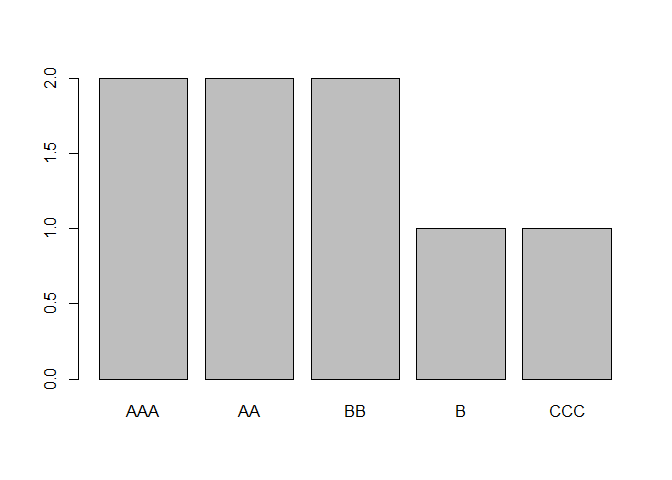
\includegraphics{Introduction_to_R_for_Finance_files/figure-latex/unnamed-chunk-21-1.pdf}
\#\#\#\#Bucketing a numeric variable into a factor Your old friend Dan
sent you a list of 50 AAA rated bonds called AAA\_rank, with each bond
having an additional number from 1-100 describing how profitable he
thinks that bond will be (100 being the most profitable). You are
interested in doing further analysis on his suggestions, but first it
would be nice if the bonds were bucketed by their ranking somehow. This
would help you create groups of bonds, from least profitable to most
profitable, to more easily analyze them.

This is a great example of creating a factor from a numeric vector. The
easiest way to do this is to use cut(). Below, Dan's 1-100 ranking is
bucketed into 5 evenly spaced groups. Note that the ( in the factor
levels means we do not include the number beside it in that group, and
the {]} means that we do include that number in the group.

\begin{Shaded}
\begin{Highlighting}[]
\NormalTok{AAA_rank<-}\KeywordTok{c}\NormalTok{(}\DecValTok{31}\NormalTok{,}\DecValTok{48}\NormalTok{,}\DecValTok{100}\NormalTok{,}\DecValTok{53}\NormalTok{,}\DecValTok{85}\NormalTok{,}\DecValTok{73}\NormalTok{,}\DecValTok{62}\NormalTok{,}\DecValTok{74}\NormalTok{,}\DecValTok{42}\NormalTok{,}\DecValTok{38}\NormalTok{,}\DecValTok{97}\NormalTok{,}\DecValTok{61}\NormalTok{,}\DecValTok{48}\NormalTok{,}\DecValTok{86}\NormalTok{,}\DecValTok{44}\NormalTok{,}\DecValTok{9}\NormalTok{,}\DecValTok{43}\NormalTok{,}\DecValTok{18}\NormalTok{,}\DecValTok{62}\NormalTok{,}\DecValTok{31}\NormalTok{,}\DecValTok{48}\NormalTok{,}\DecValTok{100}\NormalTok{,}\DecValTok{53}\NormalTok{,}\DecValTok{85}\NormalTok{,}\DecValTok{73}\NormalTok{,}\DecValTok{62}\NormalTok{,}\DecValTok{74}\NormalTok{,}\DecValTok{42}\NormalTok{,}\DecValTok{38}\NormalTok{,}\DecValTok{97}\NormalTok{,}\DecValTok{61}\NormalTok{,}\DecValTok{48}\NormalTok{,}\DecValTok{86}\NormalTok{,}\DecValTok{44}\NormalTok{,}\DecValTok{9}\NormalTok{,}\DecValTok{43}\NormalTok{,}\DecValTok{18}\NormalTok{,}\DecValTok{62}\NormalTok{,}\DecValTok{31}\NormalTok{,}\DecValTok{48}\NormalTok{,}\DecValTok{100}\NormalTok{,}\DecValTok{53}\NormalTok{,}\DecValTok{85}\NormalTok{,}\DecValTok{73}\NormalTok{,}\DecValTok{62}\NormalTok{,}\DecValTok{74}\NormalTok{,}\DecValTok{42}\NormalTok{,}\DecValTok{38}\NormalTok{,}\DecValTok{97}\NormalTok{,}\DecValTok{61}\NormalTok{,}\DecValTok{48}\NormalTok{,}\DecValTok{86}\NormalTok{,}\DecValTok{44}\NormalTok{,}\DecValTok{9}\NormalTok{,}\DecValTok{43}\NormalTok{,}\DecValTok{18}\NormalTok{,}\DecValTok{62}\NormalTok{)}
\NormalTok{AAA_factor <-}\StringTok{ }\KeywordTok{cut}\NormalTok{(}\DataTypeTok{x =}\NormalTok{ AAA_rank, }\DataTypeTok{breaks =} \KeywordTok{c}\NormalTok{(}\DecValTok{0}\NormalTok{, }\DecValTok{20}\NormalTok{, }\DecValTok{40}\NormalTok{, }\DecValTok{60}\NormalTok{, }\DecValTok{80}\NormalTok{, }\DecValTok{100}\NormalTok{))}
\KeywordTok{head}\NormalTok{(AAA_factor)}
\end{Highlighting}
\end{Shaded}

\begin{verbatim}
## [1] (20,40]  (40,60]  (80,100] (40,60]  (80,100] (60,80] 
## Levels: (0,20] (20,40] (40,60] (60,80] (80,100]
\end{verbatim}

\begin{Shaded}
\begin{Highlighting}[]
\CommentTok{# Create 4 buckets for AAA_rank using cut()}
\NormalTok{AAA_factor <-}\StringTok{ }\KeywordTok{cut}\NormalTok{(}\DataTypeTok{x =}\NormalTok{ AAA_rank, }\DataTypeTok{breaks =} \KeywordTok{c}\NormalTok{(}\DecValTok{0}\NormalTok{,}\DecValTok{25}\NormalTok{,}\DecValTok{50}\NormalTok{,}\DecValTok{75}\NormalTok{,}\DecValTok{100}\NormalTok{))}

\CommentTok{# Rename the levels }
\KeywordTok{levels}\NormalTok{(AAA_factor)<-}\KeywordTok{c}\NormalTok{(}\StringTok{"low"}\NormalTok{,}\StringTok{"medium"}\NormalTok{,}\StringTok{"high"}\NormalTok{,}\StringTok{"very_high"}\NormalTok{)}

\CommentTok{# Print AAA_factor}
\NormalTok{AAA_factor}
\end{Highlighting}
\end{Shaded}

\begin{verbatim}
##  [1] medium    medium    very_high high      very_high high      high     
##  [8] high      medium    medium    very_high high      medium    very_high
## [15] medium    low       medium    low       high      medium    medium   
## [22] very_high high      very_high high      high      high      medium   
## [29] medium    very_high high      medium    very_high medium    low      
## [36] medium    low       high      medium    medium    very_high high     
## [43] very_high high      high      high      medium    medium    very_high
## [50] high      medium    very_high medium    low       medium    low      
## [57] high     
## Levels: low medium high very_high
\end{verbatim}

\begin{Shaded}
\begin{Highlighting}[]
\CommentTok{# Plot AAA_factor}
\KeywordTok{plot}\NormalTok{(AAA_factor)}
\end{Highlighting}
\end{Shaded}

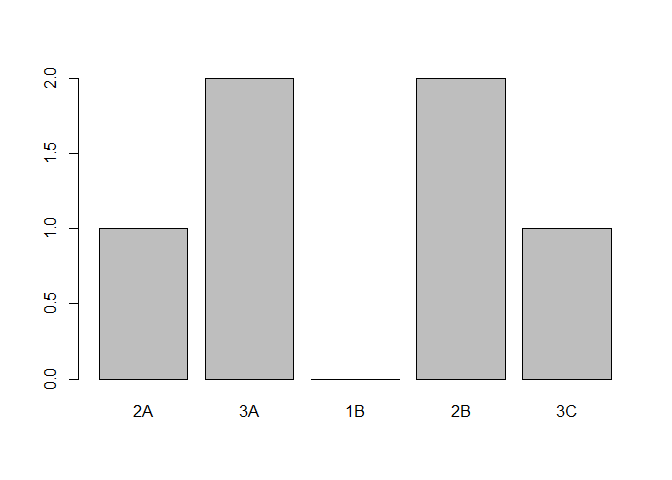
\includegraphics{Introduction_to_R_for_Finance_files/figure-latex/unnamed-chunk-22-1.pdf}
Create an ordered factor Look at the plot created over on the right. It
looks great, but look at the order of the bars! No order was specified
when you created the factor, so, when R tried to plot it, it just placed
the levels in alphabetical order. By now, you know that there is an
order to credit ratings, and your plots should reflect that!

As a reminder, the order of credit ratings from least risky to most
risky is:

AAA, AA, A, BBB, BB, B, CCC, CC, C, D To order your factor, there are
two options.

When creating a factor, specify ordered = TRUE and add unique levels in
order from least to greatest:

\begin{Shaded}
\begin{Highlighting}[]
\CommentTok{# Use unique() to find unique words}
\KeywordTok{unique}\NormalTok{(credit_rating)}
\end{Highlighting}
\end{Shaded}

\begin{verbatim}
## [1] "BB"  "AAA" "AA"  "CCC" "B"
\end{verbatim}

\begin{Shaded}
\begin{Highlighting}[]
\CommentTok{# Create an ordered factor}
\NormalTok{credit_factor_ordered <-}\StringTok{ }\KeywordTok{factor}\NormalTok{(credit_rating, }\DataTypeTok{ordered =} \OtherTok{TRUE}\NormalTok{, }\DataTypeTok{levels =} \KeywordTok{c}\NormalTok{(}\StringTok{"AAA"}\NormalTok{,}\StringTok{"AA"}\NormalTok{,}\StringTok{"BB"}\NormalTok{,}\StringTok{"B"}\NormalTok{,}\StringTok{"CCC"}\NormalTok{))}

\CommentTok{# Plot credit_factor_ordered}
\KeywordTok{plot}\NormalTok{(credit_factor_ordered)}
\end{Highlighting}
\end{Shaded}

\includegraphics{Introduction_to_R_for_Finance_files/figure-latex/unnamed-chunk-23-1.pdf}

Subsetting a factor You can subset factors in a similar way that you
subset vectors. As usual, {[} {]} is the key! However, R has some
interesting behavior when you want to remove a factor level from your
analysis. For example, what if you wanted to remove the AAA bond from
your portfolio?

credit\_factor

{[}1{]} AAA AA A BBB AA BBB A\\
Levels: BBB \textless{} A \textless{} AA \textless{} AAA

credit\_factor{[}-1{]}

{[}1{]} AA A BBB AA BBB A\\
Levels: BBB \textless{} A \textless{} AA \textless{} AAA R removed the
AAA bond at the first position, but left the AAA level behind! If you
were to plot this, you would end up with the bar chart over to the
right. A better plan would have been to tell R to drop the AAA level
entirely. To do that, add drop = TRUE:

credit\_factor{[}-1, drop = TRUE{]}

{[}1{]} AA A BBB AA BBB A\\
Levels: BBB \textless{} A \textless{} AA

\begin{Shaded}
\begin{Highlighting}[]
\CommentTok{# Remove the A bonds at positions 3 and 7. Don't drop the A level.}
\NormalTok{keep_level <-}\StringTok{ }\NormalTok{credit_factor[}\OperatorTok{-}\KeywordTok{c}\NormalTok{(}\DecValTok{3}\NormalTok{,}\DecValTok{7}\NormalTok{)]}

\CommentTok{# Plot keep_level}
\KeywordTok{plot}\NormalTok{(keep_level)}
\end{Highlighting}
\end{Shaded}

\includegraphics{Introduction_to_R_for_Finance_files/figure-latex/unnamed-chunk-24-1.pdf}

\begin{Shaded}
\begin{Highlighting}[]
\CommentTok{# Remove the A bonds at positions 3 and 7. Drop the A level.}
\NormalTok{drop_level <-credit_factor[}\OperatorTok{-}\KeywordTok{c}\NormalTok{(}\DecValTok{3}\NormalTok{,}\DecValTok{7}\NormalTok{),drop=}\StringTok{"TRUE"}\NormalTok{]}

\CommentTok{# Plot drop_level}
\KeywordTok{plot}\NormalTok{(drop_level)}
\end{Highlighting}
\end{Shaded}

\includegraphics{Introduction_to_R_for_Finance_files/figure-latex/unnamed-chunk-24-2.pdf}
stringsAsFactors Do you remember back in the data frame chapter when you
used str() on your cash data frame? This was the output:

str(cash)

`data.frame': 3 obs. of 3 variables: \$ company : Factor w/ 2 levels
``A'',``B'': 1 1 2 \$ cash\_flow: num 100 200 300 \$ year : num 1 3 2
See how the company column has been converted to a factor? R's default
behavior when creating data frames is to convert all characters into
factors. This has caused countless novice R users a headache trying to
figure out why their character columns are not working properly, but not
you! You will be prepared!

\begin{Shaded}
\begin{Highlighting}[]
\CommentTok{# Variables}
\NormalTok{credit_rating <-}\StringTok{ }\KeywordTok{c}\NormalTok{(}\StringTok{"AAA"}\NormalTok{, }\StringTok{"A"}\NormalTok{, }\StringTok{"BB"}\NormalTok{)}
\NormalTok{bond_owners <-}\StringTok{ }\KeywordTok{c}\NormalTok{(}\StringTok{"Dan"}\NormalTok{, }\StringTok{"Tom"}\NormalTok{, }\StringTok{"Joe"}\NormalTok{)}

\CommentTok{# Create the data frame of character vectors, bonds}
\NormalTok{bonds <-}\KeywordTok{data.frame}\NormalTok{(credit_rating,bond_owners,}\DataTypeTok{stringsAsFactors =} \OtherTok{FALSE}\NormalTok{)}


\CommentTok{# Use str() on bonds}
\KeywordTok{str}\NormalTok{(bonds)}
\end{Highlighting}
\end{Shaded}

\begin{verbatim}
## 'data.frame':    3 obs. of  2 variables:
##  $ credit_rating: chr  "AAA" "A" "BB"
##  $ bond_owners  : chr  "Dan" "Tom" "Joe"
\end{verbatim}

\begin{Shaded}
\begin{Highlighting}[]
\CommentTok{# Create a factor column in bonds called credit_factor from credit_rating}
\NormalTok{bonds}\OperatorTok{$}\NormalTok{credit_factor <-}\StringTok{ }\KeywordTok{factor}\NormalTok{(bonds}\OperatorTok{$}\NormalTok{credit_rating, }\DataTypeTok{ordered =} \OtherTok{TRUE}\NormalTok{, }\DataTypeTok{levels =} \KeywordTok{c}\NormalTok{(}\StringTok{"AAA"}\NormalTok{,}\StringTok{"A"}\NormalTok{,}\StringTok{"BB"}\NormalTok{))}

\CommentTok{# Use str() on bonds again}
\KeywordTok{str}\NormalTok{(bonds)}
\end{Highlighting}
\end{Shaded}

\begin{verbatim}
## 'data.frame':    3 obs. of  3 variables:
##  $ credit_rating: chr  "AAA" "A" "BB"
##  $ bond_owners  : chr  "Dan" "Tom" "Joe"
##  $ credit_factor: Ord.factor w/ 3 levels "AAA"<"A"<"BB": 1 2 3
\end{verbatim}

Create a list Just like a grocery list, lists in R can be used to hold
together items of different data types. Creating a list is, you guessed
it, as simple as using the list() function. You could say that a list is
a kind of super data type: you can store practically any piece of
information in it! Create a list like so:

words \textless{}- c(``I \textless{}3 R'') numbers \textless{}- c(42,
24)

my\_list \textless{}- list(words, numbers)

my\_list

{[}{[}1{]}{]}{[}1{]} ``I \textless{}3 R''

{[}{[}2{]}{]}{[}1{]} 42 24 Below, you will create

\begin{Shaded}
\begin{Highlighting}[]
\CommentTok{# List components}
\NormalTok{name <-}\StringTok{ "Apple and IBM"}
\NormalTok{apple <-}\StringTok{ }\KeywordTok{c}\NormalTok{(}\FloatTok{109.49}\NormalTok{, }\FloatTok{109.90}\NormalTok{, }\FloatTok{109.11}\NormalTok{, }\FloatTok{109.95}\NormalTok{, }\FloatTok{111.03}\NormalTok{)}
\NormalTok{ibm <-}\StringTok{ }\KeywordTok{c}\NormalTok{(}\FloatTok{159.82}\NormalTok{, }\FloatTok{160.02}\NormalTok{, }\FloatTok{159.84}\NormalTok{, }\FloatTok{160.35}\NormalTok{, }\FloatTok{164.79}\NormalTok{)}
\NormalTok{cor_matrix <-}\StringTok{ }\KeywordTok{cor}\NormalTok{(}\KeywordTok{cbind}\NormalTok{(apple, ibm))}

\CommentTok{# Create a list}
\NormalTok{portfolio <-}\StringTok{ }\KeywordTok{list}\NormalTok{(name,apple,ibm,cor_matrix)}

\CommentTok{# View your first list}
\NormalTok{portfolio}
\end{Highlighting}
\end{Shaded}

\begin{verbatim}
## [[1]]
## [1] "Apple and IBM"
## 
## [[2]]
## [1] 109.49 109.90 109.11 109.95 111.03
## 
## [[3]]
## [1] 159.82 160.02 159.84 160.35 164.79
## 
## [[4]]
##           apple       ibm
## apple 1.0000000 0.9131575
## ibm   0.9131575 1.0000000
\end{verbatim}

Named lists Knowing how forgetful you are, you decide it would be
important to add names to your list so you can remember what each
element is describing. There are two ways to do this!

You could name the elements as you create the list with the form name =
value:

my\_list \textless{}- list(my\_words = words, my\_numbers = numbers) Or,
if the list was already created, you could use names():

my\_list \textless{}- list(words, numbers) names(my\_list) \textless{}-
c(``my\_words'', ``my\_numbers'') Both would result in:

my\_list

\$my\_words {[}1{]} ``I \textless{}3 R''

\$my\_numbers {[}1{]} 42 24

\begin{Shaded}
\begin{Highlighting}[]
\CommentTok{# Add names to your portfolio}
\KeywordTok{names}\NormalTok{(portfolio)<-}\KeywordTok{c}\NormalTok{(}\StringTok{"portfolio_name"}\NormalTok{, }\StringTok{"apple"}\NormalTok{, }\StringTok{"ibm"}\NormalTok{, }\StringTok{"correlation"}\NormalTok{)}

\CommentTok{# Print portfolio}
\NormalTok{portfolio}
\end{Highlighting}
\end{Shaded}

\begin{verbatim}
## $portfolio_name
## [1] "Apple and IBM"
## 
## $apple
## [1] 109.49 109.90 109.11 109.95 111.03
## 
## $ibm
## [1] 159.82 160.02 159.84 160.35 164.79
## 
## $correlation
##           apple       ibm
## apple 1.0000000 0.9131575
## ibm   0.9131575 1.0000000
\end{verbatim}

Access elements in a list Subsetting a list is similar to subsetting a
vector or data frame, with one extra useful operation.

To access the elements in the list, use {[} {]}. This will always return
another list.

my\_list{[}1{]}

\$my\_words {[}1{]} ``I \textless{}3 R''

my\_list{[}c(1,2){]}

\$my\_words {[}1{]} ``I \textless{}3 R''

\$my\_numbers {[}1{]} 42 24 To pull out the data inside each element of
your list, use {[}{[} {]}{]}.

my\_list{[}{[}1{]}{]}

{[}1{]} ``I \textless{}3 R'' If your list is named, you can use the \$
operator: my\_list\$my\_words. This is the same as using {[}{[} {]}{]}
to return the inner data.

\begin{Shaded}
\begin{Highlighting}[]
\CommentTok{# Second and third elements of portfolio}
\NormalTok{portfolio[}\KeywordTok{c}\NormalTok{(}\DecValTok{2}\NormalTok{,}\DecValTok{3}\NormalTok{)]}
\end{Highlighting}
\end{Shaded}

\begin{verbatim}
## $apple
## [1] 109.49 109.90 109.11 109.95 111.03
## 
## $ibm
## [1] 159.82 160.02 159.84 160.35 164.79
\end{verbatim}

\begin{Shaded}
\begin{Highlighting}[]
\CommentTok{# Use $ to get the correlation data}
\NormalTok{portfolio}\OperatorTok{$}\NormalTok{correlation}
\end{Highlighting}
\end{Shaded}

\begin{verbatim}
##           apple       ibm
## apple 1.0000000 0.9131575
## ibm   0.9131575 1.0000000
\end{verbatim}

Adding to a list Once you create a list, you aren't stuck with it
forever. You can add new elements to it whenever you want! Say you want
to add your friend Dan's favorite movie to your list. You can do so
using \$ like you did when adding new columns to data frames.

my\_list\$dans\_movie \textless{}- ``StaR Wars''

my\_list

\$my\_words {[}1{]} ``I \textless{}3 R''

\$my\_numbers {[}1{]} 42 24

\$dans\_movie {[}1{]} ``StaR Wars'' You could have also used c() to add
another element to the list: c(my\_list, dans\_movie = ``StaR Wars'').
This can be useful if you want to add multiple elements to your list at
once.

\begin{Shaded}
\begin{Highlighting}[]
\CommentTok{# Add weight: 20% Apple, 80% IBM}
\NormalTok{portfolio}\OperatorTok{$}\NormalTok{weight <-}\StringTok{ }\KeywordTok{c}\NormalTok{(}\DataTypeTok{apple =} \FloatTok{0.2}\NormalTok{, }\DataTypeTok{ibm =} \FloatTok{0.8}\NormalTok{)}

\CommentTok{# Print portfolio}
\NormalTok{portfolio}
\end{Highlighting}
\end{Shaded}

\begin{verbatim}
## $portfolio_name
## [1] "Apple and IBM"
## 
## $apple
## [1] 109.49 109.90 109.11 109.95 111.03
## 
## $ibm
## [1] 159.82 160.02 159.84 160.35 164.79
## 
## $correlation
##           apple       ibm
## apple 1.0000000 0.9131575
## ibm   0.9131575 1.0000000
## 
## $weight
## apple   ibm 
##   0.2   0.8
\end{verbatim}

\begin{Shaded}
\begin{Highlighting}[]
\CommentTok{# Change the weight variable: 30% Apple, 70% IBM}
\NormalTok{portfolio}\OperatorTok{$}\NormalTok{weight<-}\StringTok{ }\KeywordTok{c}\NormalTok{(}\DataTypeTok{apple =} \FloatTok{0.3}\NormalTok{, }\DataTypeTok{ibm =} \FloatTok{0.7}\NormalTok{)}

\CommentTok{# Print portfolio to see the changes}
\NormalTok{portfolio}
\end{Highlighting}
\end{Shaded}

\begin{verbatim}
## $portfolio_name
## [1] "Apple and IBM"
## 
## $apple
## [1] 109.49 109.90 109.11 109.95 111.03
## 
## $ibm
## [1] 159.82 160.02 159.84 160.35 164.79
## 
## $correlation
##           apple       ibm
## apple 1.0000000 0.9131575
## ibm   0.9131575 1.0000000
## 
## $weight
## apple   ibm 
##   0.3   0.7
\end{verbatim}

Removing from a list The natural next step is to learn how to remove
elements from a list. You decide that even though Dan is your best
friend, you don't want his info in your list. To remove dans\_movie:

my\_list\$dans\_movie \textless{}- NULL

my\_list

\$my\_words {[}1{]} ``I \textless{}3 R''

\$my\_numbers {[}1{]} 42 24 Using NULL is the easiest way to remove an
element from your list! If your list is not named, you can also remove
elements by position using my\_list{[}1{]} \textless{}- NULL or
my\_list{[}{[}1{]}{]} \textless{}- NULL

\begin{Shaded}
\begin{Highlighting}[]
\CommentTok{# Take a look at portfolio}
\NormalTok{portfolio}
\end{Highlighting}
\end{Shaded}

\begin{verbatim}
## $portfolio_name
## [1] "Apple and IBM"
## 
## $apple
## [1] 109.49 109.90 109.11 109.95 111.03
## 
## $ibm
## [1] 159.82 160.02 159.84 160.35 164.79
## 
## $correlation
##           apple       ibm
## apple 1.0000000 0.9131575
## ibm   0.9131575 1.0000000
## 
## $weight
## apple   ibm 
##   0.3   0.7
\end{verbatim}

\begin{Shaded}
\begin{Highlighting}[]
\CommentTok{# Remove the microsoft stock prices from your portfolio}
\NormalTok{portfolio}\OperatorTok{$}\NormalTok{microsoft<-}\OtherTok{NULL}
\NormalTok{portfolio}
\end{Highlighting}
\end{Shaded}

\begin{verbatim}
## $portfolio_name
## [1] "Apple and IBM"
## 
## $apple
## [1] 109.49 109.90 109.11 109.95 111.03
## 
## $ibm
## [1] 159.82 160.02 159.84 160.35 164.79
## 
## $correlation
##           apple       ibm
## apple 1.0000000 0.9131575
## ibm   0.9131575 1.0000000
## 
## $weight
## apple   ibm 
##   0.3   0.7
\end{verbatim}

Split it Often, you will have data for multiple groups together in one
data frame. The cash data frame was an example of this back in Chapter
3. There were cash\_flow and year columns for two groups (companies A
and B). What if you wanted to split up this data frame into two separate
data frames divided by company? In the next exercise, you will explore
why you might want to do this, but first let's explore how to make this
happen using the split() function.

Create a grouping to split on, and use split() to create a list of two
data frames.

grouping \textless{}- cash\$company split\_cash \textless{}- split(cash,
grouping)

split\_cash

\$A company cash\_flow year 1 A 1000 1 2 A 4000 3 3 A 550 4

\$B company cash\_flow year 4 B 1500 1 5 B 1100 2 6 B 750 4 7 B 6000 5

\begin{Shaded}
\begin{Highlighting}[]
\CommentTok{# Define grouping from year}
\NormalTok{grouping <-}\StringTok{ }\NormalTok{cash}\OperatorTok{$}\NormalTok{year}

\CommentTok{# Split cash on your new grouping}
\NormalTok{split_cash <-}\StringTok{ }\KeywordTok{split}\NormalTok{(cash,grouping)}

\CommentTok{# Look at your split_cash list}
\NormalTok{split_cash}
\end{Highlighting}
\end{Shaded}

\begin{verbatim}
## $`1`
##   cash_flow year quarter_cash double_year present_value
## 1      1000    1          250           2       952.381
## 4      1500    1          375           2      1428.571
## 
## $`2`
##   cash_flow year quarter_cash double_year present_value
## 5      1100    2          275           4      997.7324
## 
## $`3`
##   cash_flow year quarter_cash double_year present_value
## 2      4000    3         1000           6       3455.35
## 
## $`4`
##   cash_flow year quarter_cash double_year present_value
## 3       550    4        137.5           8      452.4864
## 6       750    4        187.5           8      617.0269
## 
## $`5`
##   cash_flow year quarter_cash double_year present_value
## 7      6000    5         1500          10      4701.157
\end{verbatim}

\begin{Shaded}
\begin{Highlighting}[]
\CommentTok{# Unsplit split_cash to get the original data back.}
\NormalTok{original_cash <-}\StringTok{ }\KeywordTok{unsplit}\NormalTok{(split_cash,grouping)}

\CommentTok{# Print original_cash}
\NormalTok{original_cash}
\end{Highlighting}
\end{Shaded}

\begin{verbatim}
##   cash_flow year quarter_cash double_year present_value
## 1      1000    1        250.0           2      952.3810
## 2      4000    3       1000.0           6     3455.3504
## 3       550    4        137.5           8      452.4864
## 4      1500    1        375.0           2     1428.5714
## 5      1100    2        275.0           4      997.7324
## 6       750    4        187.5           8      617.0269
## 7      6000    5       1500.0          10     4701.1570
\end{verbatim}

Split-Apply-Combine A common data science problem is to split your data
frame by a grouping, apply some transformation to each group, and then
recombine those pieces back into one data frame. This is such a common
class of problems in R that it has been given the name
split-apply-combine. In Intermediate R for Finance, you will explore a
number of these problems and functions that are useful when solving
them, but, for now, let's do a simple example.

Suppose, for the cash data frame, you are interested in doubling the
cash\_flow for company A, and tripling it for company B:

grouping \textless{}- cash\$company split\_cash \textless{}- split(cash,
grouping)

\section{We can access each list element's cash\_flow column
by:}\label{we-can-access-each-list-elements-cash_flow-column-by}

split\_cash\(A\)cash\_flow {[}1{]} 1000 4000 550

split\_cash\(A\)cash\_flow \textless{}- split\_cash\(A\)cash\_flow * 2
split\_cash\(B\)cash\_flow \textless{}- split\_cash\(B\)cash\_flow * 3

new\_cash \textless{}- unsplit(split\_cash, grouping) Take a look again
at how you access the cash\_flow column. The first \$ is to access the A
element of the split\_cash list. The second \$ is to access the
cash\_flow column of the data frame in A.

\begin{Shaded}
\begin{Highlighting}[]
\CommentTok{# Print split_cash}
\NormalTok{split_cash}
\end{Highlighting}
\end{Shaded}

\begin{verbatim}
## $`1`
##   cash_flow year quarter_cash double_year present_value
## 1      1000    1          250           2       952.381
## 4      1500    1          375           2      1428.571
## 
## $`2`
##   cash_flow year quarter_cash double_year present_value
## 5      1100    2          275           4      997.7324
## 
## $`3`
##   cash_flow year quarter_cash double_year present_value
## 2      4000    3         1000           6       3455.35
## 
## $`4`
##   cash_flow year quarter_cash double_year present_value
## 3       550    4        137.5           8      452.4864
## 6       750    4        187.5           8      617.0269
## 
## $`5`
##   cash_flow year quarter_cash double_year present_value
## 7      6000    5         1500          10      4701.157
\end{verbatim}

\begin{Shaded}
\begin{Highlighting}[]
\CommentTok{# Print the cash_flow column of B in split_cash}
\NormalTok{split_cash}\OperatorTok{$}\NormalTok{B}\OperatorTok{$}\NormalTok{cash_flow}
\end{Highlighting}
\end{Shaded}

\begin{verbatim}
## NULL
\end{verbatim}

\begin{Shaded}
\begin{Highlighting}[]
\CommentTok{# Set the cash_flow column of company A in split_cash to 0}
\NormalTok{split_cash}\OperatorTok{$}\NormalTok{A}\OperatorTok{$}\NormalTok{cash_flow <-}\DecValTok{0}

\CommentTok{# Use the grouping to unsplit split_cash}
\NormalTok{cash_no_A <-}\StringTok{ }\KeywordTok{unsplit}\NormalTok{(split_cash,grouping)}

\CommentTok{# Print cash_no_A}
\NormalTok{cash_no_A}
\end{Highlighting}
\end{Shaded}

\begin{verbatim}
##   cash_flow year quarter_cash double_year present_value
## 1      1000    1        250.0           2      952.3810
## 2      4000    3       1000.0           6     3455.3504
## 3       550    4        137.5           8      452.4864
## 4      1500    1        375.0           2     1428.5714
## 5      1100    2        275.0           4      997.7324
## 6       750    4        187.5           8      617.0269
## 7      6000    5       1500.0          10     4701.1570
\end{verbatim}

Attributes You have made it to the last exercise in the course!
Congrats! Let's finish up with an easy one.

Attributes are a bit of extra metadata about your data structure. Some
of the most common attributes are: row names and column names,
dimensions, and class. You can use the attributes() function to return a
list of attributes about the object you pass in. To access a specific
attribute, you can use the attr() function.

Exploring the attributes of cash:

attributes(cash)

\$names {[}1{]} ``company'' ``cash\_flow'' ``year''

\$row.names {[}1{]} 1 2 3 4 5 6 7

\$class {[}1{]} ``data.frame''

attr(cash, which = ``names'')

{[}1{]} ``company'' ``cash\_flow'' ``year''

\begin{Shaded}
\begin{Highlighting}[]
\CommentTok{# my_matrix and my_factor}
\NormalTok{my_matrix <-}\StringTok{ }\KeywordTok{matrix}\NormalTok{(}\KeywordTok{c}\NormalTok{(}\DecValTok{1}\NormalTok{,}\DecValTok{2}\NormalTok{,}\DecValTok{3}\NormalTok{,}\DecValTok{4}\NormalTok{,}\DecValTok{5}\NormalTok{,}\DecValTok{6}\NormalTok{), }\DataTypeTok{nrow =} \DecValTok{2}\NormalTok{, }\DataTypeTok{ncol =} \DecValTok{3}\NormalTok{)}
\KeywordTok{rownames}\NormalTok{(my_matrix) <-}\StringTok{ }\KeywordTok{c}\NormalTok{(}\StringTok{"Row1"}\NormalTok{, }\StringTok{"Row2"}\NormalTok{)}
\KeywordTok{colnames}\NormalTok{(my_matrix) <-}\StringTok{ }\KeywordTok{c}\NormalTok{(}\StringTok{"Col1"}\NormalTok{, }\StringTok{"Col2"}\NormalTok{, }\StringTok{"Col3"}\NormalTok{)}

\NormalTok{my_factor <-}\StringTok{ }\KeywordTok{factor}\NormalTok{(}\KeywordTok{c}\NormalTok{(}\StringTok{"A"}\NormalTok{, }\StringTok{"A"}\NormalTok{, }\StringTok{"B"}\NormalTok{), }\DataTypeTok{ordered =}\NormalTok{ T, }\DataTypeTok{levels =} \KeywordTok{c}\NormalTok{(}\StringTok{"A"}\NormalTok{, }\StringTok{"B"}\NormalTok{))}

\CommentTok{# attributes of my_matrix}
\KeywordTok{attributes}\NormalTok{(my_matrix)}
\end{Highlighting}
\end{Shaded}

\begin{verbatim}
## $dim
## [1] 2 3
## 
## $dimnames
## $dimnames[[1]]
## [1] "Row1" "Row2"
## 
## $dimnames[[2]]
## [1] "Col1" "Col2" "Col3"
\end{verbatim}

\begin{Shaded}
\begin{Highlighting}[]
\CommentTok{# Just the dim attribute of my_matrix}
\KeywordTok{attr}\NormalTok{(my_matrix,}\StringTok{"dim"}\NormalTok{)}
\end{Highlighting}
\end{Shaded}

\begin{verbatim}
## [1] 2 3
\end{verbatim}

\begin{Shaded}
\begin{Highlighting}[]
\CommentTok{# attributes of my_factor}
\KeywordTok{attributes}\NormalTok{(my_factor)}
\end{Highlighting}
\end{Shaded}

\begin{verbatim}
## $levels
## [1] "A" "B"
## 
## $class
## [1] "ordered" "factor"
\end{verbatim}


\end{document}
